\documentclass[ngerman,a4paper,twoside]{article}

%\usepackage{epsfig,varioref,titlesec,latexsym,amssymb,amsmath,fancybox,graphicx}
\usepackage{varioref,titlesec,latexsym,amssymb,amsmath,fancybox,graphicx}
\usepackage{xcolor,relsize}
%\usepackage{babel}

\usepackage{hyperref}
\hypersetup{
  colorlinks,
  linkcolor=blue,
  filecolor=blue,
  urlcolor=blue,	
  citecolor=blue,
  plainpages=false,
  hypertexnames=false,
}

\usepackage[nottoc]{tocbibind}
\usepackage{soul}
\usepackage{color}
\usepackage{epstopdf}
\epstopdfsetup{update} % only regenerate pdf files when eps file is newer

\usepackage[scaled]{helvet} %Helvetica-Fonts z.B. phvb
\renewcommand*\familydefault{\sfdefault} % sans serif as default
\newfont{\myheadfont}{phvb scaled \magstep4}

\usepackage{fancyhdr}
\usepackage{lmodern}
\usepackage{amsmath}
\usepackage{mytitlepage}

\hyphenpenalty=500

%\DeclareMathSizes{10}{8}{8}{7}   % For size 10 text
%\DeclareMathSizes{12}{11}{10}{8}   % For size 10 text
%\DeclareMathSizes{11}{19}{13}{9}   % For size 11 text
%\DeclareMathSizes{12}{20}{14}{10}  % For size 12 text

% Layout Seitenkopf
%\addtolength{\headwidth}{\marginparsep}
%\addtolength{\headwidth}{\marginparwidth}

\setcounter{secnumdepth}{3}
\setcounter{tocdepth}{3}

\newfont{\bss}{bessy scaled \magstep 4}

\setlength{\unitlength}{1cm}

\clubpenalty=10000
\widowpenalty = 10000
\displaywidowpenalty = 10000

\textwidth 16. cm
\topmargin .0 cm
\textheight 22.5 cm
\parskip 0.3 cm
\sloppy %Gegenteil von \fussy
\oddsidemargin 0.0 cm
\evensidemargin 0.0 cm
\parindent=0.cm

\begin{document}

\thispagestyle{empty}

\begin{center}
\LARGE \textbf{PyBrill\\ Tutorial} \\[1cm]

\textbf{ \Large Michael Scheer} \\[0.cm]
%\textbf{ \Large Helmholtz-Zentrum Berlin} \\[0.75cm]

\textbf{ \Large \today }\\
\begin{figure}[htb]
   \vspace*{2.5cm}
   \centering
   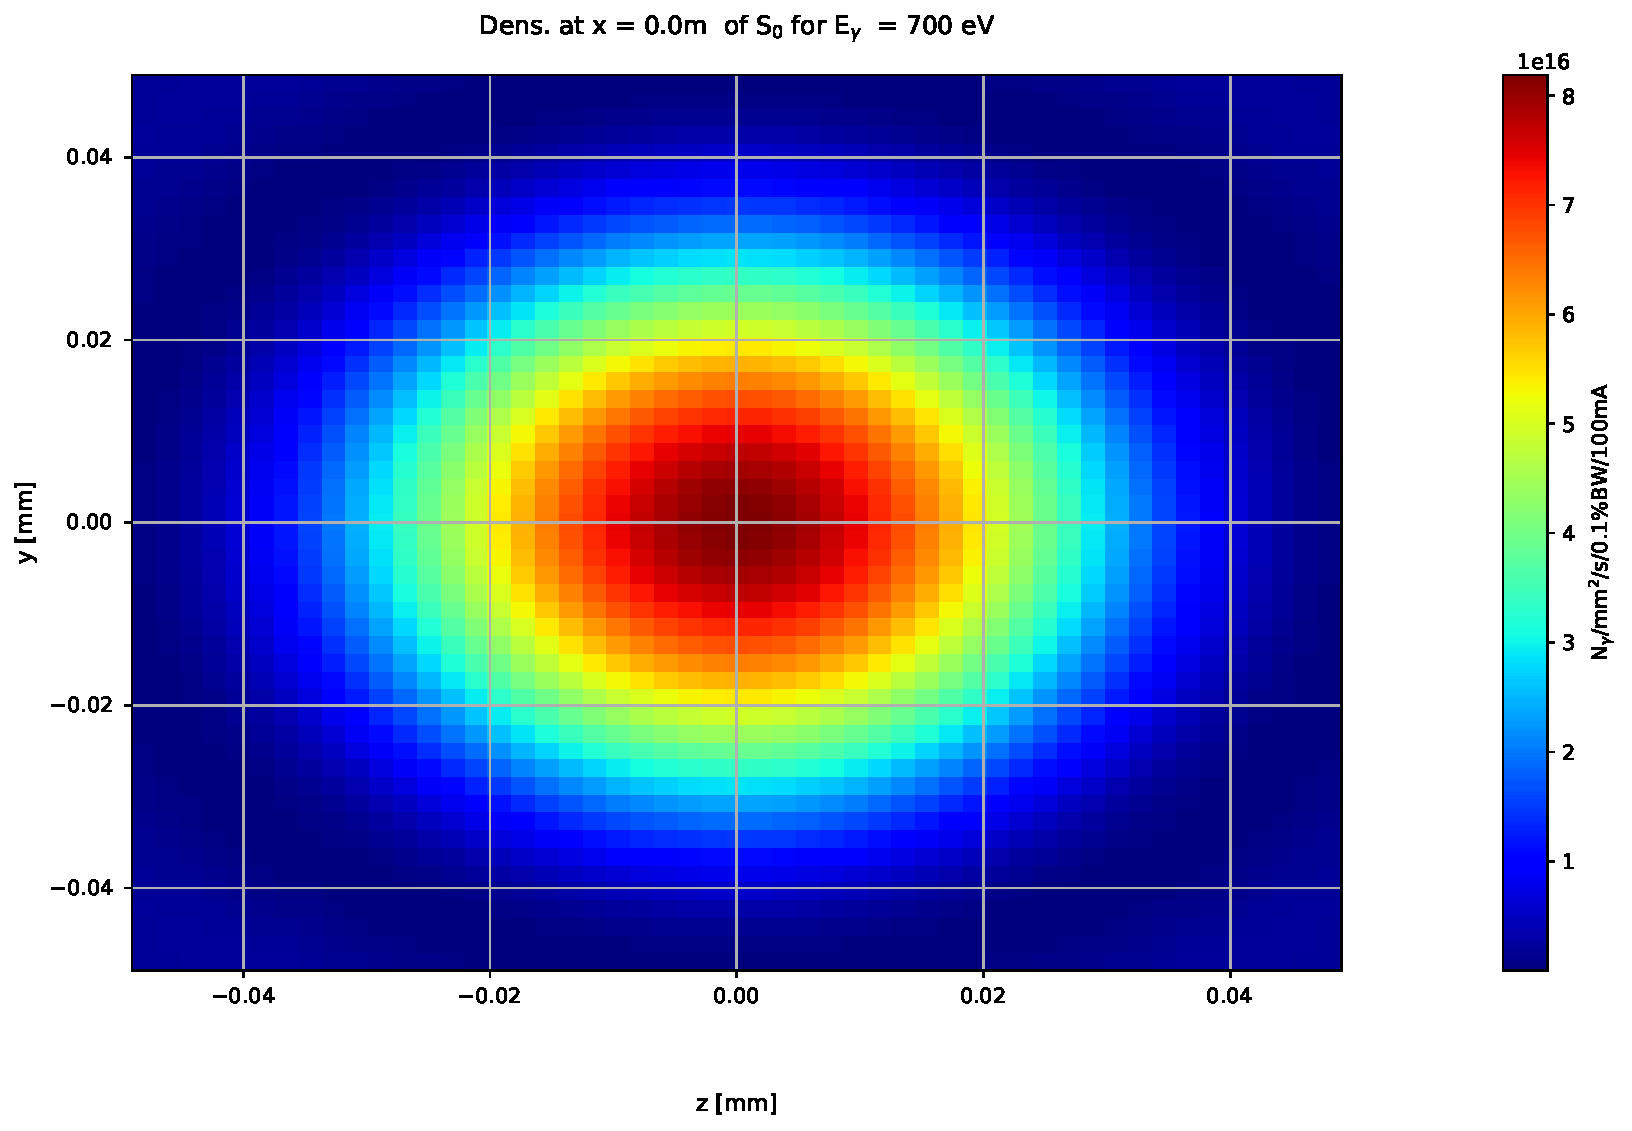
\includegraphics[width=0.75\textwidth]
   {pictures/cover.pdf}
\end{figure}
\end{center}

%\newpage
%\thispagestyle{empty}
%{~}

%+PATCH,//BRILL/TEX
%+DECK,abbrevs,T=LATEX.
\newcommand{\vitemt}[2]{
\begin{center}
{
\setlength{\fboxrule}{3pt}
\fcolorbox{schwachgrau}{hellgrau}
  {\color{black}
    \setlength{\fboxrule}{0pt}
    \framebox[0.5\textwidth]{#1 \hfill}
    \colorbox{white}{\color{black} #2}
  }
}
\end{center}
}

\newcommand{\vitem}[2]{
\begin{center}
{
\setlength{\fboxrule}{3pt}
\fcolorbox{schwachgrau}{hellgrau}
  {\color{black}
    \setlength{\fboxrule}{0pt}
    \framebox[0.25\textwidth]{\small #1 \hfill}
    \framebox[0.2\textwidth]{\hfill
      \colorbox{white}{\color{black} \small #2}
    }
  }
}
\end{center}
}

\newcommand{\bsp}{\hspace{-0.2cm}}

\newcommand{\git}[1]{\textbf{\color{grau}\textit{#1}} \color{black}}
\newcommand{\gits}[1]{\textbf{\color{grau}\textit{\textsmaller[0.3]{#1}}} \color{black}}
\newcommand{\gitse}[1]{\textbf{\color{grau}\textit{\textsmaller[0.3]{#1}}}\color{black}}
\newcommand{\gite}[1]{\textbf{\color{grau}\textit{#1}}\color{black}}

\newcommand{\gti}[1]{\textbf{\color{grau}\textit{#1}} \color{black}}
\newcommand{\gtis}[1]{\textbf{\color{grau}\textit{\textsmaller[0.3]{#1}}} \color{black}}
\newcommand{\gtise}[1]{\textbf{\color{grau}\textit{\textsmaller[0.3]{#1}}}\color{black}}
\newcommand{\gtie}[1]{\textbf{\color{grau}\textit{#1}}\color{black}}

\newcommand{\witem}[1]{
  \begin{center}
    \colorbox{schwachgrau}{
      \colorbox{hellgrau}{
      \color{grau}
      \framebox[0.45\textwidth]{\color{black} \small #1}
      }
    }
  \end{center}
}

\newcommand{\witemrot}[1]{
  \begin{center}
    \colorbox{yellow}{
      \colorbox{red}{
      \color{red}
      \framebox[0.45\textwidth]{\color{white} \small #1}
      }
    }
  \end{center}
}

\newcommand{\witems}[1]{
  \begin{center}
    \colorbox{yellow}{
      \colorbox{blue}{
      \color{blue}
      \framebox[0.5\textwidth]{\color{white} #1}
      }
    }
  \end{center}
}

\newcommand{\witemss}[1]{
  \begin{center}
    \colorbox{yellow}{
      \colorbox{blue}{
      \color{blue}
      \framebox[0.5\textwidth]{\color{white} #1}
      }
    }
  \end{center}
}

\newcommand{\witemsss}[1]{
  \begin{center}
    \colorbox{yellow}{
      \colorbox{blue}{
      \color{blue}
      \framebox[0.5\textwidth]{\color{white} #1}
      }
    }
  \end{center}
}

\newcommand{\ryellow}[1]{
  \begin{center}
    \colorbox{yellow}{\color{yellow}
      \framebox[0.6\textwidth]{\color{black} \small #1}
    }
  \end{center}
}
\newcommand{\rorange}[1]{
  \begin{center}
    \colorbox{orange}{\color{orange}
      \framebox[0.6\textwidth]{\color{black} \small #1}
    }
  \end{center}
}
\newcommand{\ryellows}[1]{
  \begin{center}
    \colorbox{yellow}{\color{yellow}
      \framebox[0.55\textwidth]{\color{black} \small #1}
    }
  \end{center}
}
\newcommand{\roranges}[1]{
  \begin{center}
    \colorbox{orange}{\color{orange}
      \framebox[0.55\textwidth]{\color{black} \small #1}
    }
  \end{center}
}
\newcommand{\rmft}[1]{\ryellow{magnetic field and trajectory}}
\newcommand{\rby}[1]{\ryellows{By(x)}}
\newcommand{\rbys}[1]{\ryellows{By(x) with observed sources of radiation}}
\newcommand{\rnz}[1]{\ryellows{nz(x)}}
\newcommand{\rnzs}[1]{\ryellows{nz(x) with observed sources of radiation}}
\newcommand{\rnzp}[1]{\ryellows{nzp(x)}}
\newcommand{\rnzps}[1]{\ryellows{nzp(x) with observed sources of radiation}}

\newcommand{\witemold}[1]{
  \begin{center}
    \colorbox{yellow}{
      \colorbox{blue}{
      \color{blue}
      \framebox[0.6\textwidth]{\color{white} \small #1}
      }
    }
  \end{center}
}

\newcommand{\witemsold}[1]{
  \begin{center}
    \colorbox{yellow}{
      \colorbox{blue}{
      \color{blue}
      \framebox[0.575\textwidth]{\color{white} \small #1}
      }
    }
  \end{center}
}

\newcommand{\witemssold}[1]{
  \begin{center}
    \colorbox{yellow}{
      \colorbox{blue}{
      \color{blue}
      \framebox[0.55\textwidth]{\color{white} \small #1}
      }
    }
  \end{center}
}

\newcommand{\witemsssold}[1]{
  \begin{center}
    \colorbox{yellow}{
      \colorbox{blue}{
      \color{blue}
      \framebox[0.50\textwidth]{\color{white} \small #1}
      }
    }
  \end{center}
}

\definecolor{darkslategray}{rgb}{0.18, 0.31, 0.31}
\definecolor{gray}{rgb}{0.18, 0.31, 0.31}

\definecolor{orange}{rgb}{1.,0.8,0.4} % rgb
\definecolor{hellgrau}{gray}{0.9}
\definecolor{schwachgrau}{gray}{0.95}
\definecolor{grau}{gray}{0.4}
\definecolor{dunkelgrau}{gray}{0.2}

\newcommand{\vitemold}[2]{
\begin{center}
  \colorbox{yellow}{
    \color{yellow}
    \colorbox{white}{
      \color{white}
      \framebox[0.6\textwidth]{
        \colorbox{blue}{\color{white} \small #1}
        \hfill \
        \colorbox{blue}{\color{white} \small #2}
      }
    }
  }
\end{center}
}

\newcommand{\grau}{\color{grau}}
\newcommand{\dunkelgrau}{\color{dunkelgrau}}
\newcommand{\schwarz}{\color{black}}

\newcommand{\Lin}{{\textit{\grau{\textbf{Linux~}}}}}
\newcommand{\bash}{{\textit{\grau{\textbf{bash~}}}}}
\newcommand{\Win}{{\textit{\grau{\textbf{Windows~}}}}}
\newcommand{\Lie}{{\textit{\grau{\textbf{Linux}}}}}
\newcommand{\Wine}{{\textit{\grau{\textbf{Windows}}}}}

\newcommand{\PyB}{{\textit{\grau{\textbf{PyBrill~}}}}}
\newcommand{\pyB}{{\textit{\grau{\textbf{pyBrill~}}}}}
\newcommand{\pyBe}{{\textit{\grau{\textbf{pyBrill}}}}}

\newcommand{\PB}{{\textit{\grau{\textbf{PyBrill~}}}}}
\newcommand{\pB}{{\textit{\grau{\textbf{pyBrill~}}}}}
\newcommand{\pBe}{{\textit{\grau{\textbf{pyBrill}}}}}

\newcommand{\bri}{{\textit{\grau{\textbf{brill~}}}}}
\newcommand{\brie}{{\textit{\grau{\textbf{brill}}}}}

\newcommand{\sta}{{\textit{\grau{\textbf{stage~}}}}}
\newcommand{\stae}{{\textit{\grau{\textbf{stage}}}}}

\newcommand{\bin}{{\textit{\grau{\textbf{bin}}}}}
\newcommand{\bine}{{\textit{\grau{\textbf{bin}}}}}

\newcommand{\wdir}{{\textit{\grau{\textbf{working directory~}}}}}
\newcommand{\wdire}{{\textit{\grau{\textbf{working directory}}}}}

\newcommand{\Py}{{\textit{\grau{\textbf{Python~}}}}}
\newcommand{\Pye}{{\textit{\grau{\textbf{Python}}}}}
\newcommand{\F}{{\textit{\grau{\textbf{FORTRAN~}}}}}
\newcommand{\Fe}{{\textit{\grau{\textbf{FORTRAN}}}}}

\newcommand{\Urp}{{\textit{\grau{\textbf{Urad\_phase~}}}}}
\newcommand{\urp}{{\textit{\grau{\textbf{urad\_phase~}}}}}
\newcommand{\urpe}{{\textit{\grau{\textbf{urad\_phase}}}}}

\newcommand{\Unam}{{\textit{\grau{\textbf{Urad\_phase.nam~}}}}}
\newcommand{\unam}{{\textit{\grau{\textbf{urad\_phase.nam~}}}}}
\newcommand{\uname}{{\textit{\grau{\textbf{urad\_phase.nam}}}}}

\newcommand{\mhb}{{\textit{\grau \textsmaller[2]{\textbf{WAVE.mhb~}}}}}
\newcommand{\mhbe}{{\textit{\grau \textsmaller[2]{\textbf{WAVE.mhb}}}}}
\newcommand{\dw}{{\textit{\grau \textsmaller[1.]{\$WAVE}}}}
\newcommand{\WSH}{{\textit{\grau\textsmaller[2]{\textbf{WAVESHOP~}}}}}
\newcommand{\WSHE}{{\textit{\grau\textsmaller[2]{\textbf{WAVESHOP}}}}}

\newcommand{\scap}[1]{\textit{\textsmaller[1]{\textbf{\grau #1}}}}
\newcommand{\cbox}[1]{\vspace{0.1cm}\hspace{1cm}\parbox[c]{0.8\textwidth}{\gti{\hspace{-0.2cm}#1}}}
\newcommand{\cboxs}[1]{\hspace{1cm} \parbox[c]{0.8\textwidth}{\grau \small \gti{#1}}}
\newcommand{\cboxss}[1]{\hspace{1cm}\parbox[c]{0.8\textwidth}{\grau
\textbf{\textsmaller[2]{#1}}}}
\newcommand{\cboxsl}[1]{\parbox[c]{0.9\textwidth}{\small \gti{#1}}}
\newcommand{\hin}{\hspace{1cm}}
\newcommand{\ro}{{\textit{source \dw/shell/wave\_root.sh}}}
\newcommand{\row}{{\textit{source \dw/shell/wave\_root.sh wave}}}
\newcommand{\gui}{{\textit{source \dw/shell/wave\_root.sh gui}}}
\newcommand{\wi}{{\gtis{wave.in~}}}
\newcommand{\wie}{{\gtise{wave.in}}}
\newcommand{\wo}{{\gtis{wave.out~}}}
\newcommand{\woe}{{\gtis{wave.out}}}
\newcommand{\wvs}{{\gti{wave.wvs~}}}
\newcommand{\wpl}{{\gti{wplot~}}}
\newcommand{\wple}{{\gti{wplot \bsp}}}
\newcommand{\wpg}{{\gti{waveplot.py~}}}
\newcommand{\wro}{{\gti{WAVE.root~}}}
\newcommand{\w}{{\gti{wave}}}
\newcommand{\senv}{\gtis{. \dw/shell/set\_wave\_environment.sh}}
\newcommand{\we}{{\gtis{\dw/input/wave.examples~}}}
\newcommand{\wee}{{\gtis{\dw/input/wave.examples}}}
\newcommand{\U}{{\small UNDUMAG~}}
\newcommand{\Ue}{{\small UNDUMAG}}
\newcommand{\W}{{\small WAVE~}}
\newcommand{\We}{{\small WAVE}}
\newcommand{\WS}{{{\small WAVES~}}}
\newcommand{\R}{{\small ROOT}}
\newcommand{\ws}{{\textit{waves~}}}
%\newcommand{\wpl}{{\textit{waves.pl~}}}
%\newcommand{\wpy}{{\textit{waves.py~}}}
\newcommand{\ispecnull}{{{\scap{ISPEC=0~}}}}
\newcommand{\ispecone}{{{\scap{ISPEC=1~}}}}
\newcommand{\ispec}{{\grau \bf \scap{ISPEC~}}}
\newcommand{\imagsplnnull}{{\scap{IMAGSPLN=0~}}}
\newcommand{\imagsplnone}{{\scap{IMAGSPLN=1~}}}
\newcommand{\imagspln}{{\scap{IMAGSPLN~}}}
\newcommand{\ieneloss}{{\scap{IENELOSS~}}}
\newcommand{\xstart}{{\scap{XSTART~}}}
\newcommand{\ystart}{{\scap{YSTART~}}}
\newcommand{\zstart}{{\scap{ZSTART~}}}
\newcommand{\vxin}{{\scap{VXIN~}}}
\newcommand{\vyin}{{\scap{VYIN~}}}
\newcommand{\vzin}{{\scap{VZIN~}}}
\newcommand{\dmyenergy}{{\scap{DMYENERGY~}}}
\newcommand{\dmycurr}{{\scap{DMYCURR~}}}
\newcommand{\ienelossnull}{{\scap{IENELOSS=0~}}}
\newcommand{\ienelossone}{{\scap{IENELOSS=1~}}}
\newcommand{\dend}{{\textbf{\grau\bf\textit{\textsmaller[1]{\$END~}}}}\schwarz}
\newcommand{\dende}{{\textbf{\grau\bf\textit{\textsmaller[1]{\$END}}}}\schwarz}
\newcommand{\contrl}{{\textbf{\grau\bf\textit{\textsmaller[1]{\$CONTRL~}}}}\schwarz}
\newcommand{\contrle}{{\textbf{\grau\bf\textit{\textsmaller[1]{\$CONTRL}}}}\schwarz}
\newcommand{\halbach}{{{\scap{\$HALBACH~}}}}
\newcommand{\ellip}{{{\scap{\$ELLIP~}}}}
\newcommand{\halbasy}{{{\scap{\$HALBAS}Y~}}}

%\renewcommand{\chaptername}{}
%\renewcommand{\contentsname}{\vspace{-1cm} \center{\Large Contents} \\[-1cm]}
%\renewcommand{\bibname}{\vspace{-3cm} \Large Literature \\[-0.4cm]}
\renewcommand{\listfigurename}{\vspace{-3cm} \Large Figures \\[-0.4cm]}
\renewcommand{\listtablename}{\vspace{-3cm} \Large Tables \\[-0.4cm]}
\renewcommand{\appendixname}{Appendix}
\renewcommand{\figurename}{Fig.}
\renewcommand{\tablename}{Tab.}

\newcommand{\lchib}{\mbox{ $ \large{\bar{ \chi}} $ }}
\newcommand{\chib}{\mbox{ $ \bar{ \chi } $ }}

\newcommand{\bt}{\tilde{\beta}}
\newcommand{\bnt}{\tilde{\beta_0}}
\newcommand{\boptt}{\tilde{\beta_{opt}}}
\newcommand{\bnopt}{{\beta}_{0,opt}}
\newcommand{\bnoptt}{\tilde{\beta}_{0,opt}}
\newcommand{\et}{\tilde{\eta}}
\newcommand{\eet}{\tilde{\eta_e}}
\newcommand{\eeopt}{\eta_{e,opt}}
\newcommand{\eeoptt}{\tilde{\eta}_{e,opt}}
\newcommand{\eit}{\tilde{\eta_i}}
\newcommand{\AT}{\tilde{A}}
\newcommand{\BT}{\tilde{B}}
\newcommand{\CT}{\tilde{C}}
\newcommand{\DT}{\tilde{D}}
\newcommand{\DOPTT}{\tilde{D}_{opt}}
\newcommand{\ET}{\tilde{E}}

\newcommand{\kapitel}{\chapter}

\newcommand{\proz}{^0\!/\!_{0}}
\newcommand{\prom}{^0\!/\!_{00}}

\renewcommand{\textfraction}{0.01}
\renewcommand{\floatpagefraction}{0.01}
\renewcommand{\topfraction}{0.99}
\renewcommand{\bottomfraction}{0.99}

%\renewcommand{\figurename}{\bf Fig.}
%\renewcommand{\tablename}{\bf Tab.}

\newcommand{\fig}[8]	%  8 parameters are required:
			% #1: FIGURE width: cm
			% #2: FIGURE hight: cm
			% #3: FIGURE caption width: cm
			% #4: figure position: hERE, tOP, bOTTOM
			% #5: figure label
			% #6: figure caption (TEXT ZUM BILD)
			% #7: entry for figure caption
			% #8: Bild File (Postscript)
{
\begin{figure}[#4]
   %\vspace{0.5cm}
   \centering{
   \epsfig{file=#8,width=#1cm}
   \parbox[t]{#3cm}
       {\vspace{-0.2cm} \caption[#7]{\label{#5} #6}}
   } % centering
   \vspace{-0.65cm}
\end{figure}
}

\newcommand{\figo}[9]	% 9 parameters are required:
			% #1: FIGURE width: cm
			% #2: FIGURE caption width: cm
			% #3: vertical offset preceeding picture: cm
			% #4: vertical offset following picture: cm
			% #5: figure position: hERE, tOP, bOTTOM
			% #6: figure label
			% #7: figure caption (TEXT ZUM BILD)
			% #8: entry for figure caption
			% #9: Bild File (Postscript)
{
\begin{figure}[#5]
   \vspace{#3cm}
   \centering{
   \epsfig{file=#9,width=#1cm}
   \parbox[t]{#2cm}
       {\caption[#8]{\label{#6} #7}}
   } % centering
   \vspace{#4cm}
\end{figure}
}

\newcommand{\abb}[4]	%  4 parameters are required:
			% #1: figure label
			% #2: figure caption (TEXT ZUM BILD)
			% #3: entry for figure caption
			% #4: Bild File (Postscript)
{
\begin{figure}[htb]
   %\vspace{0.5cm}
   \centering{
   \epsfig{file=#4,width=12cm}
   \parbox[t]{12cm}
       {\caption[#3]{\label{#1} #2}}
   } % centering
   \vspace{-0.5cm}
\end{figure}
}

% *** muessen unbedingt hinter \pagestyle{fancy} stehen, da dort defaults def.
%\renewcommand{\chaptermark}[1]{\markboth{\thechapter\ #1}{}}
%\renewcommand{\sectionmark}[1]{\markright{\thesection\ #1}}
%\renewcommand{\sectionmark}[1]{\markright{\thesection}}
%\renewcommand{\chaptermark}[1]{\markboth{#1}{}}
%\renewcommand{\sectionmark}[1]{\markright{#1}}


%+PATCH,//BRILL/TEX
%+DECK,introduction,T=LATEX.

%\renewcommand*\thesection{\Roman{section}}
%\section{Introduction}

\large
\PB has been developed at BESSY for the fast and easy calculation of
spontaneous synchrotron radiation of an analytical undulator model.
This includes brilliance,
radiation field, Stokes parameters, Wigner-Distributions.
Monte-Carlo techniques allow to take emittance and energy-spread of
the electron beam into account and to generate
photons for ray-tracing.

\PB and the related software is published under the GNU General Public
License. To get pyBrill, please contact the author or get it from github:

~~~~~\gti{git clone https://github.com/MicScheer/brill.git brill}


%\newpage

\setcounter{page}{1}
\tableofcontents

%\newpage

\pagestyle{fancy}

%\lhead[\bfseries\thepage]{\bfseries\rightmark}
\lhead[\textit \thepage]{\textit \rightmark}
\chead[]{}
%\rhead[\bfseries\leftmark]{\bfseries\thepage}
\rhead[\textit \leftmark]{\textit \thepage}

\lfoot[]{}
\cfoot[
%+seq,docvers.
]{}
\rfoot[]{}

\definecolor{orange}{rgb}{1.,0.8,0.4} % rgb

\large

\include{Requirements}

%+PATCH,//BRILL/TEX
%+DECK,getting_started,T=LATEX.

\renewcommand*\thesection{\Roman{section}}
\section{Getting Started}

First, we open a terminal and clone the whole package from Github to the directory
\bri:

\cbox{git clone https://github.com/MicScheer/brill.git brill}

We call the directory \bri of \pB it's home directory and the
sub-directory \sta the working directory.

Since \urp is a standalone program, we can run it by hand, i.e. not
deploying \pBe. We change to the \wdir and run \urpe:

\cbox{
cd stage\\
../bin/urad\_phase.exe
}

The program should run and write some lines to the terminal.\\

\begin{figure}[htb]
   \centering
   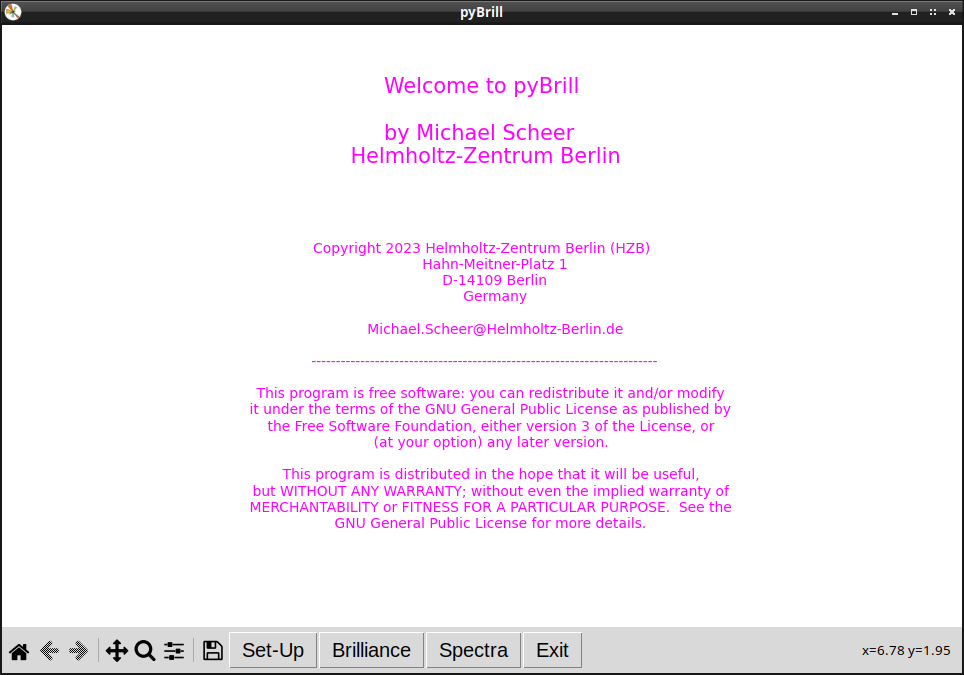
\includegraphics[width=0.8\textwidth]
   {pictures/pybrill.png}
   \caption{Start Menu of pyBrill}
   \label{gsfig1}
\end{figure}
		
\Urp reads the input data from a namelist file \uname. This file can
be edit by the user, but it also can be created by \pBe, which has
menus to set the variables, run \urpe, and plots the results.

We start \pB and try it:\\[-1.0cm]

\cbox{
python3 -i ../python/pyBrill.py
}

The size and position of the window can be controlled by editing the
first line of\\[-1.0cm]

\cbox{
ntupplot.cfg
}

The other parameters are not relevant for \pBe. An example of this file can be found
in the sub-directory \git{input} of the home directory of \pBe.

\subsection{Brilliance Calculations}

\begin{figure}[htb]
   \centering
   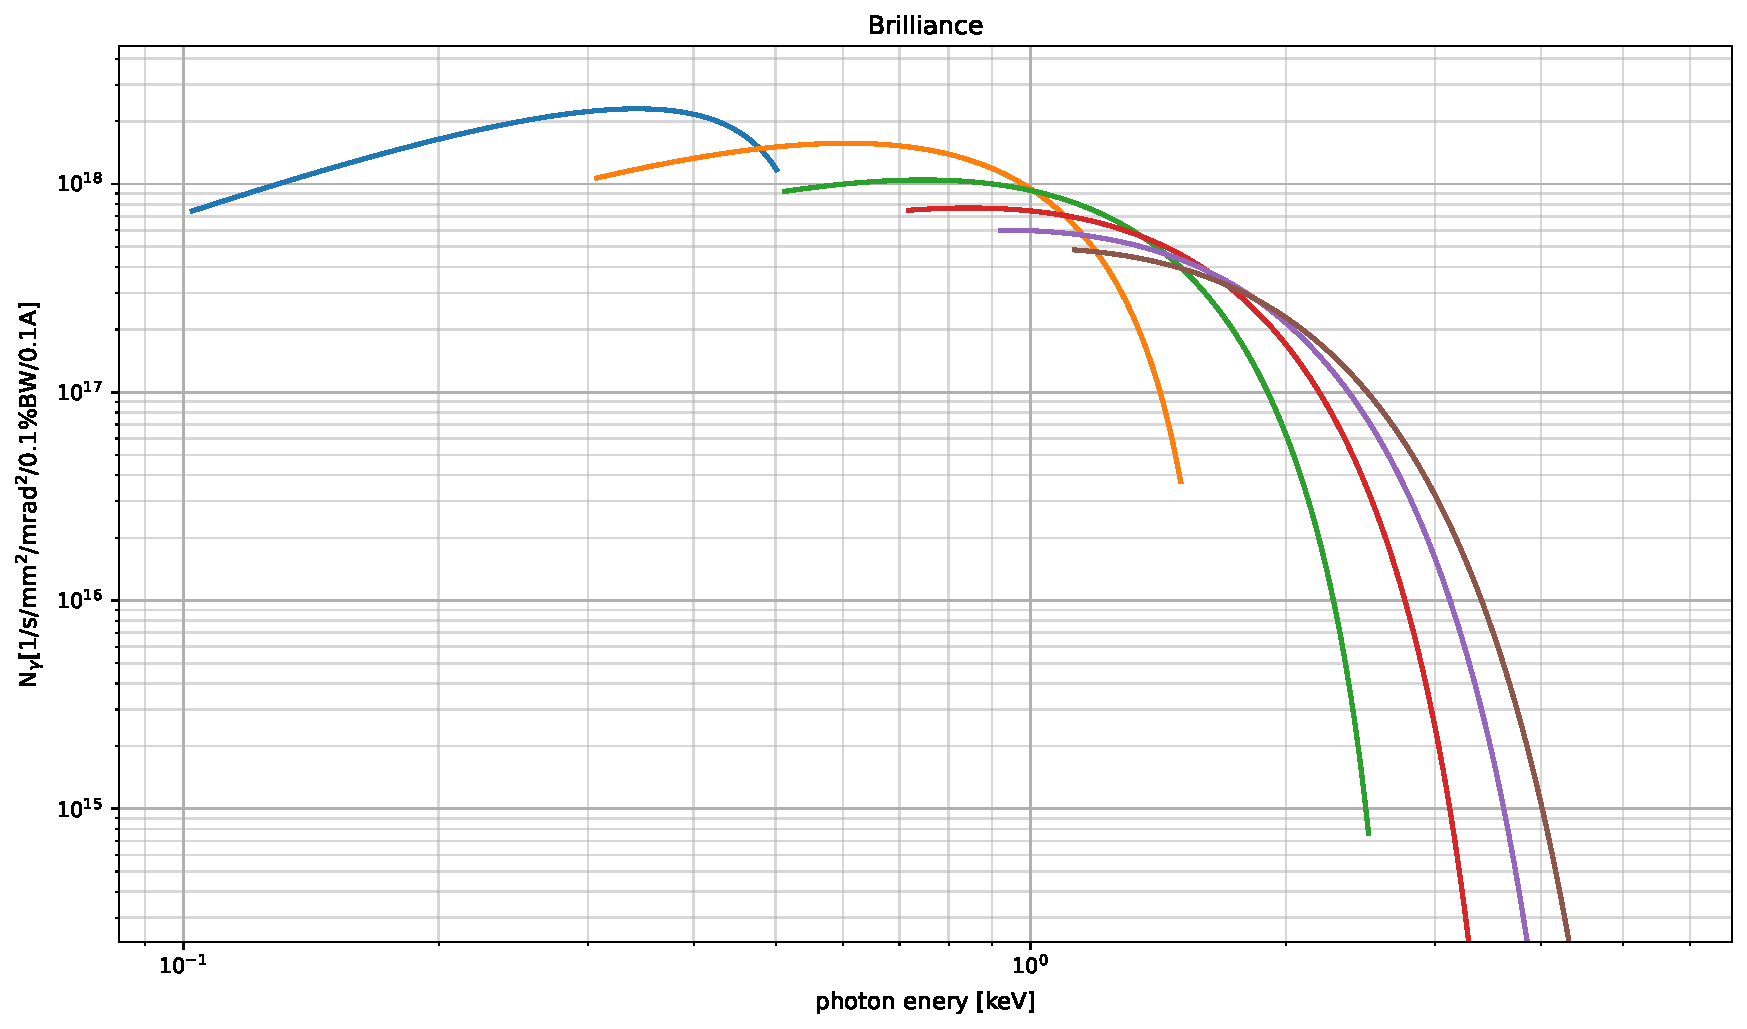
\includegraphics[width=0.8\textwidth]
   {pictures/brilliance.pdf}
   \caption{Brilliance Plot}
   \label{gsfig2}
\end{figure}

Press the button labeled \git{Brilliance} and plot the brilliance of the
undulator. As you can see in the terminal, the plotted data are
written to files. The plot itself is save as PDF-file.

To control the brilliance calculation, press the \gti{Set-Up} button
and check the menu items. The \gti{spectra} item is not used the
brilliance calculations. It is reserved for the spectra calculations
with \urpe.

The default values are set by \pB or read from a file named

\cbox{.pybrill\_last.dat}

which is written when the \gti{Exit} button of \pB is pressed. Note,
if you leave \pB by entering "q" while the focus is on the output
screen, the data are not stored.

\subsection{Spectrum Calculations}

\begin{figure}[htb]
   \centering
   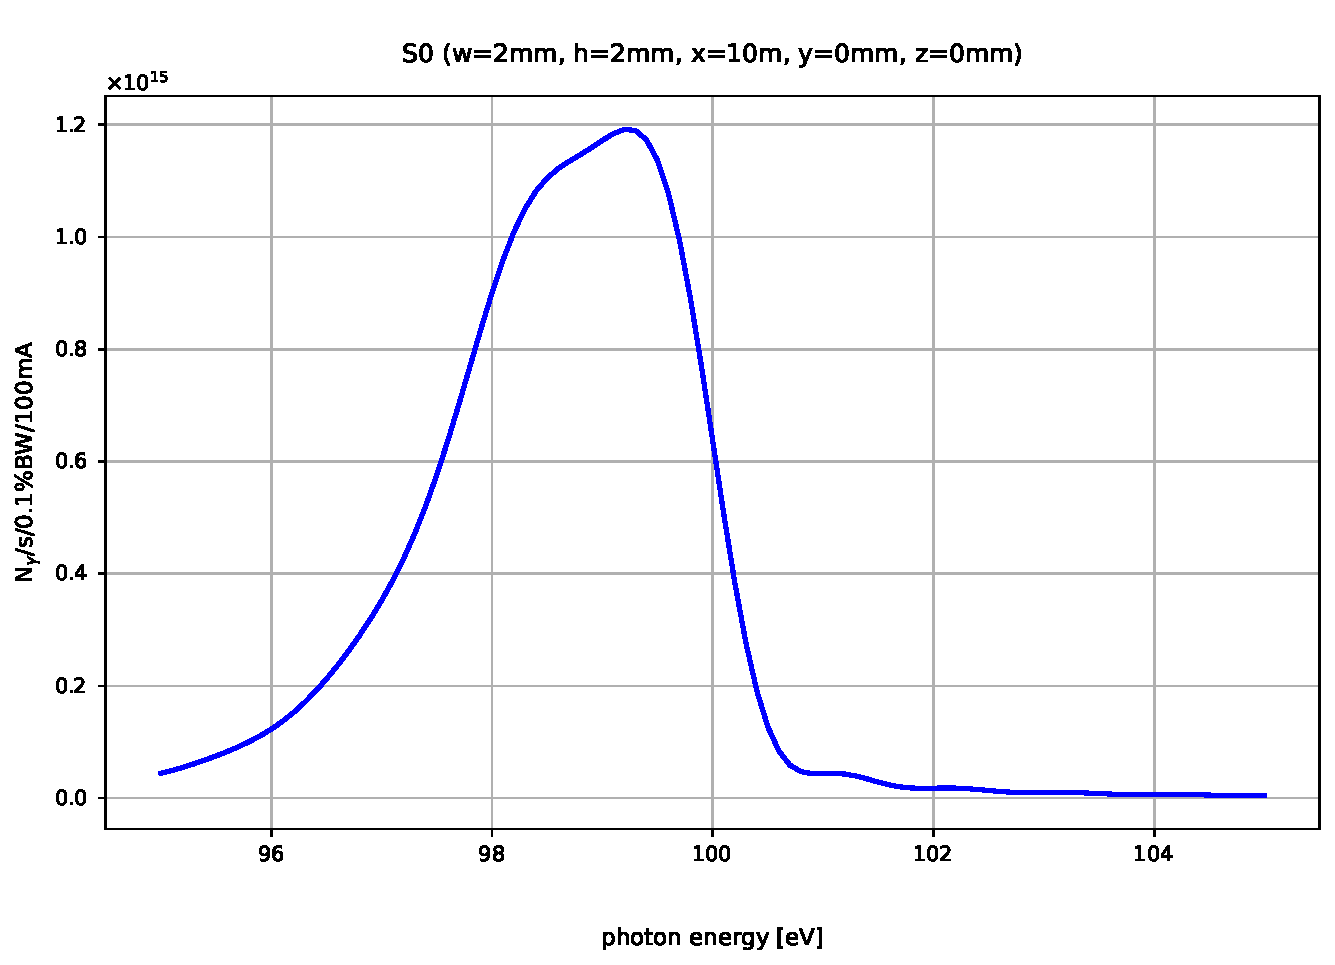
\includegraphics[width=0.7\textwidth]
   {pictures/flux.pdf}
   \caption{Flux of Undulator}
   \label{gsfig3}
\end{figure}

Press the \gti{Spectra} button, select \gite{Plot/Flux/Stokes/S0}. The
flux of the Stokes parameter \git{S0} through the rectangular pinhole
as calculated by \urp is plotted (Fig. \ref{gsfig3}).

\begin{figure}[htb]
   \centering
   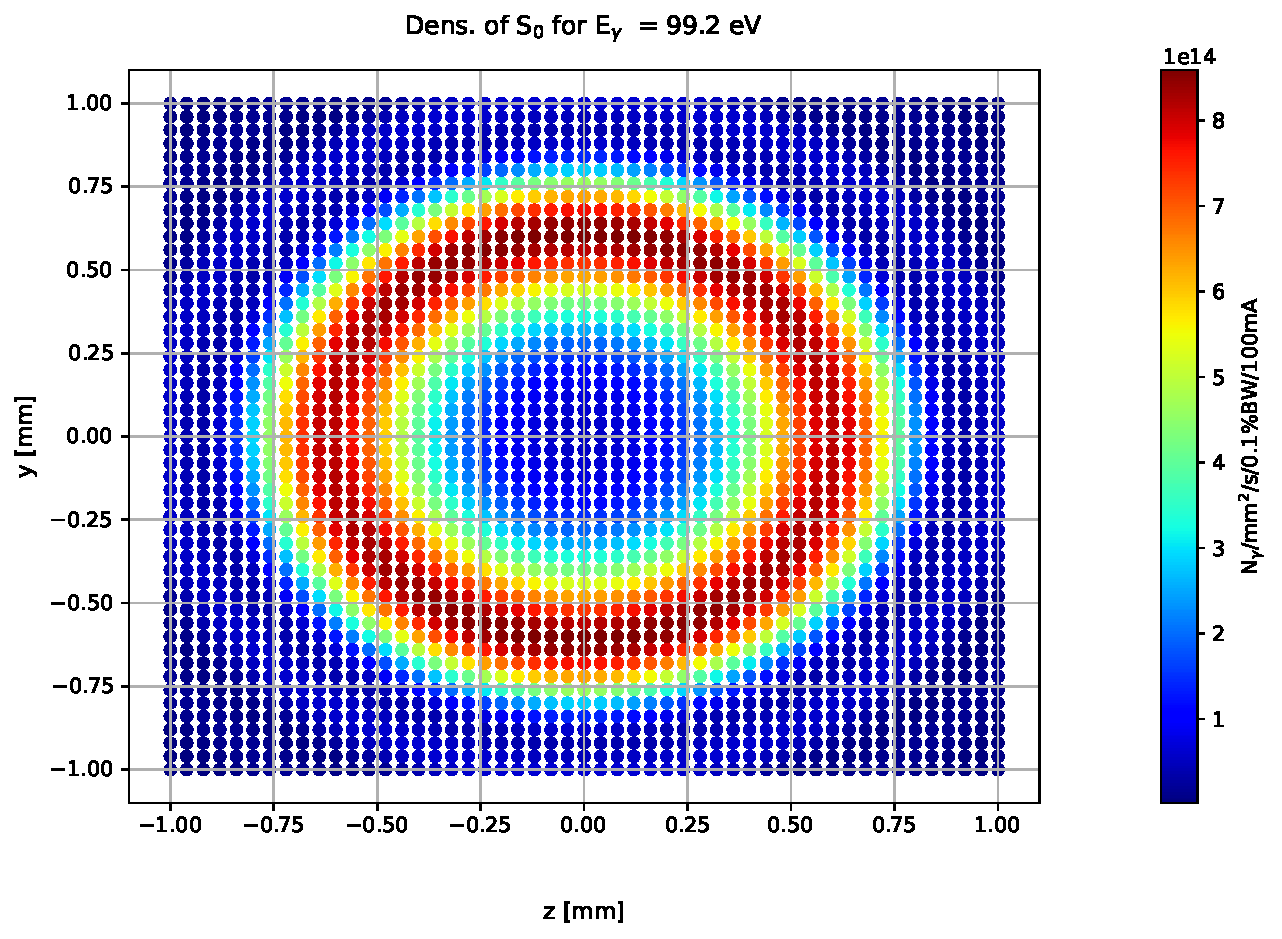
\includegraphics[width=0.7\textwidth]
   {pictures/fdpin.pdf}
   \caption{Flux-density Distribution}
   \label{gsfig4}
\end{figure}

Now, we select
\gti{Spectra/Plot/Distributions in Pinhole/Stokes/S0}
and see the flux-density distribution of \gti{S0}. The photon energy is
selected to show the distribution for the photon energy which the
maximum flux trough the pinhole.

To step through the photon energies, the arrows of the keyboard can be
used. The photon energy can also be selected from the menu

\cbox{\gti{Spectra/Plot/Distributions in Pinhole/Select E\_photon}
}


%\section{Format of Ouput Files}

The main output files of the spectrum calculations are

\cbox{
urad_phase.flx\\
urad_phase.fld\\
urad_phase.bun\\
}

\cbox{}


%+PATCH,//BRILL/TEX
%+DECK,examples,T=LATEX.

\renewcommand*\thesection{\Roman{section}}
\section{Examples}

There exsists  in the \gti{input} directory a file for every given example.

You may copy this file to

\cbox{.pybrill\_last.dat}

in the working directory, start \pB and trigger the calculations
by pressing \gti{Brilliance/Calculate} or \gtie{Spectra/Calculate}.
However, it is recommended to start with the first example and use
\git{Set-Up} to preceed to the next example.

\subsection{Basic Beam Electron Monte-Carlo}

\begin{figure}[htb]
   \centering
   \includegraphics[width=0.55\textwidth]
   {pictures/ex1\_setup.png}
   \vspace*{-0.2cm}
   \caption{\gti{Set-Up/Spectra} for example 1}
   \label{ex1fig1}
\end{figure}

Before we start, we clean up the working directory to have a well defined, reproducable
setting:

\cbox{
rm .pybrill\_last.dat\\
rm urad\_phase.bun\\
rm urad\_phase.fld\\
rm urad\_phase.flx\\
rm urad\_phase.geo\\
rm urad\_phase.nor\\
rm urad\_phase.pin\\
rm urad\_phase.run
}

We start \pBe, press \gti{Set-Up}, and set:

\cbox{
Nelec = 1000\\
Number of Photon Energies = 11\\
Min. Photon Energy = 695.0\\
Max. Photon Energy = 705.0 \\
Width of Pinhole = 1.0 \\
Height of Pinhole = 1.0
}

We close the menu and click

\cbox{Spectra/Calculate}

We see, that the calculations take about a minute, depending on your
computer.

\cbox{Spectra/Plot/Flux}

\begin{figure}[htb]
   \centering
   \includegraphics[width=0.5\textwidth]
   {pictures/ex1\_flx.pdf}
   \vspace*{-0.2cm}
   \caption{\gti{Flux spectrum}}
   \label{ex1fig2}
\end{figure}

The flux spectrum we see, stems from 1000 electrons randomly chosen in
there phase-space. Thus, the result will probably change, when we
rerun the calculations. However, in the set-up you find an option to
fix the starting seed of the random number generator. This allows to
reproduce results of a program run.

We have a look on the flux-density distribution in the pinhole (Fig.
\ref{ex1fig2}:

\cbox{Spectra/Plot/Distribution in Pinhole/Stokes/S0}

\begin{figure}[htb]
   \centering
   \includegraphics[width=0.5\textwidth]
   {pictures/ex1\_scat2d.pdf}
   \vspace*{-0.2cm}
   \caption{\gti{Flux spectrum, plotted with option 'scat2d'}}
   \label{ex1fig3}
\end{figure}

\begin{figure}[htb]
   \centering
   \includegraphics[width=0.5\textwidth]
   {pictures/ex1\_inter.pdf}
   \vspace*{-0.2cm}
   \caption{\gti{Flux spectrum, plotted with option 'inter'}}
   \label{ex1fig4}
\end{figure}

We change the plotting options by selecting:

\cbox{Spectra/Plotting Options}

and choosing 'inter' and plot the distribution again
(Fig. \ref{ex1fig3}
).

\subsection{Combining Beam Electron and Observation Point Monte-Carlo}

For a large number of electrons and many grid points, the calculation
time can increase drastically. To speed up the calculations of the
flux through the pinhole,
we select in \gti{Set-Up/Spectra}

\cbox{
Nelec = 100000\\
Each n\_th electron is recorded = 100 \\
Number of Photons Energies = 1}

We close the menu and start the calculations.

\begin{figure}[htb]
   \centering
   \includegraphics[width=0.5\textwidth]
   {pictures/ex2\_flux.pdf}
   \vspace*{-0.2cm}
   \caption{\gti{Flux through pinhole with one sigma confidence level}}
   \label{ex2flux}
\end{figure}

Now, we only have to wait some seconds due to

\cbox{Number of Photons Energies = 1}

In this mode, for each electron a single observation point is
randomly choosen in the pinhole. We see that flux spectrum shows only small statistical
uncertainty (Fig. \ref{ex2flux}).

\begin{figure}[htb]
   \centering
   \includegraphics[width=0.5\textwidth]
   {pictures/ex2\_fdpin.pdf}
   \vspace*{-0.2cm}
   \caption{\gti{Flux-density in pinhole, plotted with option 'boxes'}}
   \label{ex2fdpin}
\end{figure}

However, when we look at the distribution of the flux-density in the
pinhole, we see clearly fluctions due to this special Monte-Carlo mode (Fig.
\ref{ex2fdpin}).

But in many cases, only the spetra of the flux, the flux-density, or
the profiles of the distributions (Fig. \ref{ex2fdprof}) are of interest.

\begin{figure}[htb]
   \centering
   \includegraphics[width=0.5\textwidth]
   {pictures/ex2\_fdprof.pdf}
   \vspace*{-0.2cm}
   \caption{\gti{Profile of flux-density in pinhole}}
   \label{ex2fdprof}
\end{figure}

Also the reduced number of sampled
electrons speeds up the calculations, since the I/O is reduced.

\begin{figure}[htb]
%   \vspace*{-2.5cm}
   \centering
   \includegraphics[width=0.5\textwidth]
   {pictures/ex2\_zzp.pdf}
   \vspace*{-0.2cm}
   \caption{
   \gti{Horizontal phase-space of beam electrons sample}}
   \label{ex2zzp}
\end{figure}

To check the phase-space a sample of 1000 electrons is certainly
sufficient (Fig. \ref{ex2zzp}).

\subsection{Back Propagation of the Radiation to the Source Plane}

To calculate the source size, we propagate the radiation back to the
source plane by selecting in \gti{Set-Up/Spectra}\\

\cbox{
Nelec = 1\\
Number of Photons Energies = 0 \\
Width of Pinhole = 2.0 \\
Height of Pinhole = 2.0 \\
Number of hori. points = 101 \\
Number of vert. points = 101 \\
Propagate radiation field back to origin = 1 \\
Width of Pinhole in Plane = 0.1 \\
Height of Pinhole in Plane = 0.1 \\
Number of hori. points in Plane = 51 \\
Number of vert. points in Plane = 51
}\\

and starting the calculations. Then we switch on the statistic option in
the menu

\cbox{Spectra/Plotting options}

and plot the horizontal cut of the Stokes
$S_0$ in the menu

\cbox{Plot/Distributions of Propagated Fields}

\begin{figure}[htb]
   \centering
   \includegraphics[width=0.5\textwidth]
   {pictures/ex3\_pinhcut.pdf}
   \vspace*{-0.2cm}
   \caption{
   \gti{Horizontal cut of $S_0$ in observation plane}}
   \label{ex3pinh}
\end{figure}

For the product of the RMS values of the two plots

\begin{eqnarray*}
\sigma_r \times \sigma_{r'} &=&
\frac{\lambda}{4 \pi}
\end{eqnarray*}
	
we find

\begin{figure}[htb]
   \centering
   \includegraphics[width=0.5\textwidth]
   {pictures/ex3\_prophcut.pdf}
   \vspace*{-0.2cm}
   \caption{
   \gti{Horizontal cut of $S_0$ in source plane}}
   \label{ex3proph}
\end{figure}

\begin{eqnarray*}
0.1074 ~mm \times 0.01846 ~mm / 10~m &=&
0.1982604 ~nm
\end{eqnarray*}

We have $\lambda = 1.77 ~nm$ for $700 ~eV$, thus

\begin{eqnarray*}
\frac{1.77~nm}{4 \pi} &=& 0.141 ~ nm
\end{eqnarray*}

which underestimates the numerical value by a factor of $\sqrt{2}$.

\subsection{Generating Photons from Undulator Source for Ray-tracing}

\PyB uses the cross product of the calculated electric and magnetic
fields to generate photons as input for ray-tracing codes.

\begin{figure}[htb]
   \centering
   \includegraphics[width=0.5\textwidth]
   {pictures/ex4\_ztz.pdf}
   \vspace*{-0.2cm}
   \caption{
   \gti{Horizontal phase-space of generated photons}}
   \label{ex4ztz.pdf}
\end{figure}

Due to the applied algorithm
in this examples the photons are generated for an exact beam energy,
i.e. without energy-spread.

To generate photons for electrons with energy-spread the program must
sample the beam energy in discrete steps. The number of steps can
be set in the set-up menu.

Note, if you run the program for another beam energy by hand, to see
the effect of beam energy deviations, make shure that the undulater is
set-up such that the fields are not adjusted according to the actual
energy,
as it is done, when a fixed harmonic is selected in the undulator
set-up menu.


\include{hyphenation}

%
%+PATCH,//BRILL/TEX
%+DECK,getting_started,T=LATEX.

\renewcommand*\thesection{\Roman{section}}
\section{Getting Started}

First, we open a terminal and clone the whole package from Github to the directory
\bri:

\cbox{git clone https://github.com/MicScheer/brill.git brill}

We call the directory \bri of \pB it's home directory and the
sub-directory \sta the working directory.

Since \urp is a standalone program, we can run it by hand, i.e. not
deploying \pBe. We change to the \wdir and run \urpe:

\cbox{
cd stage\\
../bin/urad\_phase.exe
}

The program should run and write some lines to the terminal.\\

\begin{figure}[htb]
   \centering
   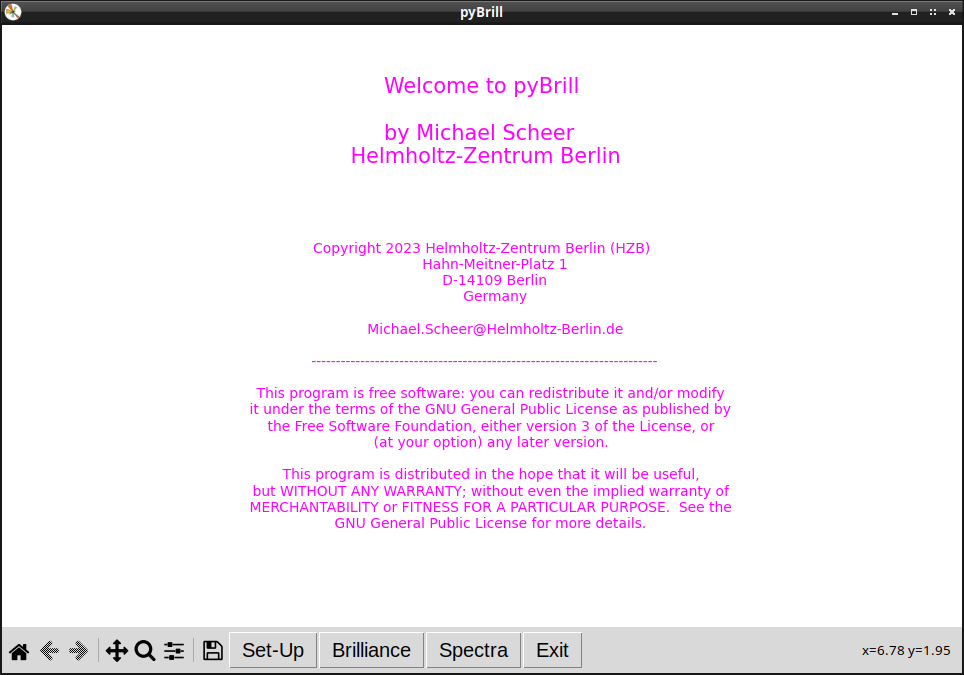
\includegraphics[width=0.8\textwidth]
   {pictures/pybrill.png}
   \caption{Start Menu of pyBrill}
   \label{gsfig1}
\end{figure}
		
\Urp reads the input data from a namelist file \uname. This file can
be edit by the user, but it also can be created by \pBe, which has
menus to set the variables, run \urpe, and plots the results.

We start \pB and try it:\\[-1.0cm]

\cbox{
python3 -i ../python/pyBrill.py
}

The size and position of the window can be controlled by editing the
first line of\\[-1.0cm]

\cbox{
ntupplot.cfg
}

The other parameters are not relevant for \pBe. An example of this file can be found
in the sub-directory \git{input} of the home directory of \pBe.

\subsection{Brilliance Calculations}

\begin{figure}[htb]
   \centering
   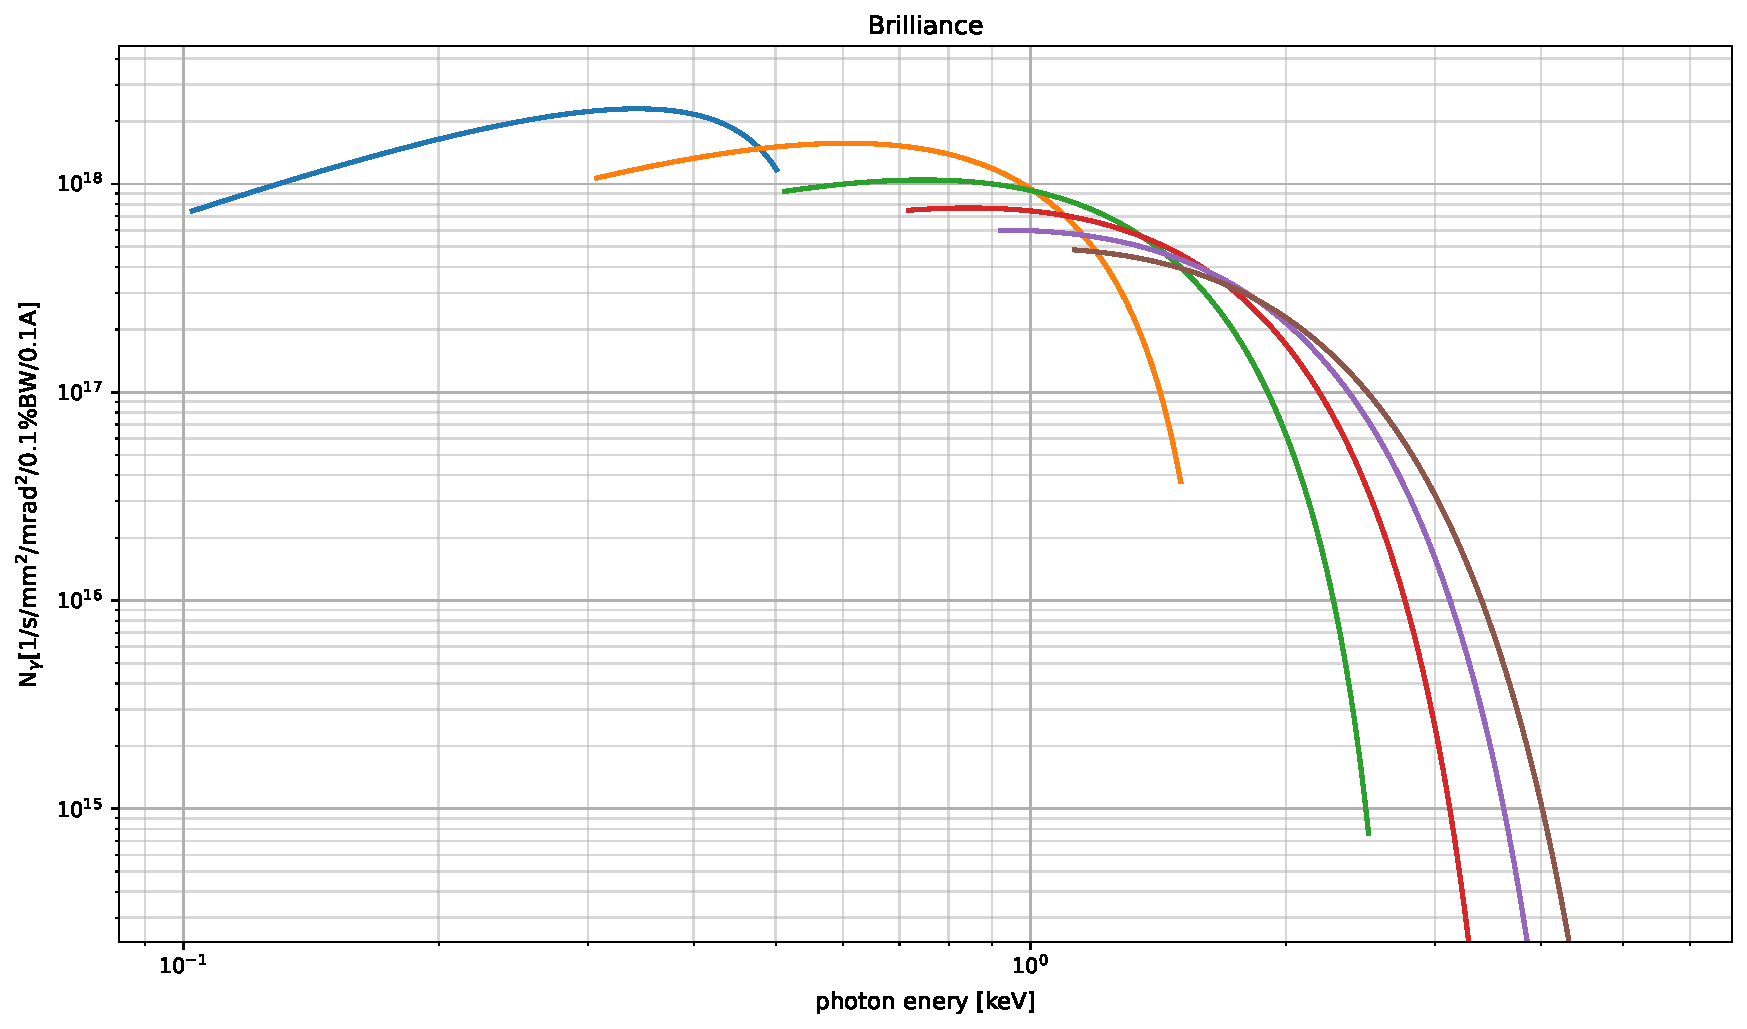
\includegraphics[width=0.8\textwidth]
   {pictures/brilliance.pdf}
   \caption{Brilliance Plot}
   \label{gsfig2}
\end{figure}

Press the button labeled \git{Brilliance} and plot the brilliance of the
undulator. As you can see in the terminal, the plotted data are
written to files. The plot itself is save as PDF-file.

To control the brilliance calculation, press the \gti{Set-Up} button
and check the menu items. The \gti{spectra} item is not used the
brilliance calculations. It is reserved for the spectra calculations
with \urpe.

The default values are set by \pB or read from a file named

\cbox{.pybrill\_last.dat}

which is written when the \gti{Exit} button of \pB is pressed. Note,
if you leave \pB by entering "q" while the focus is on the output
screen, the data are not stored.

\subsection{Spectrum Calculations}

\begin{figure}[htb]
   \centering
   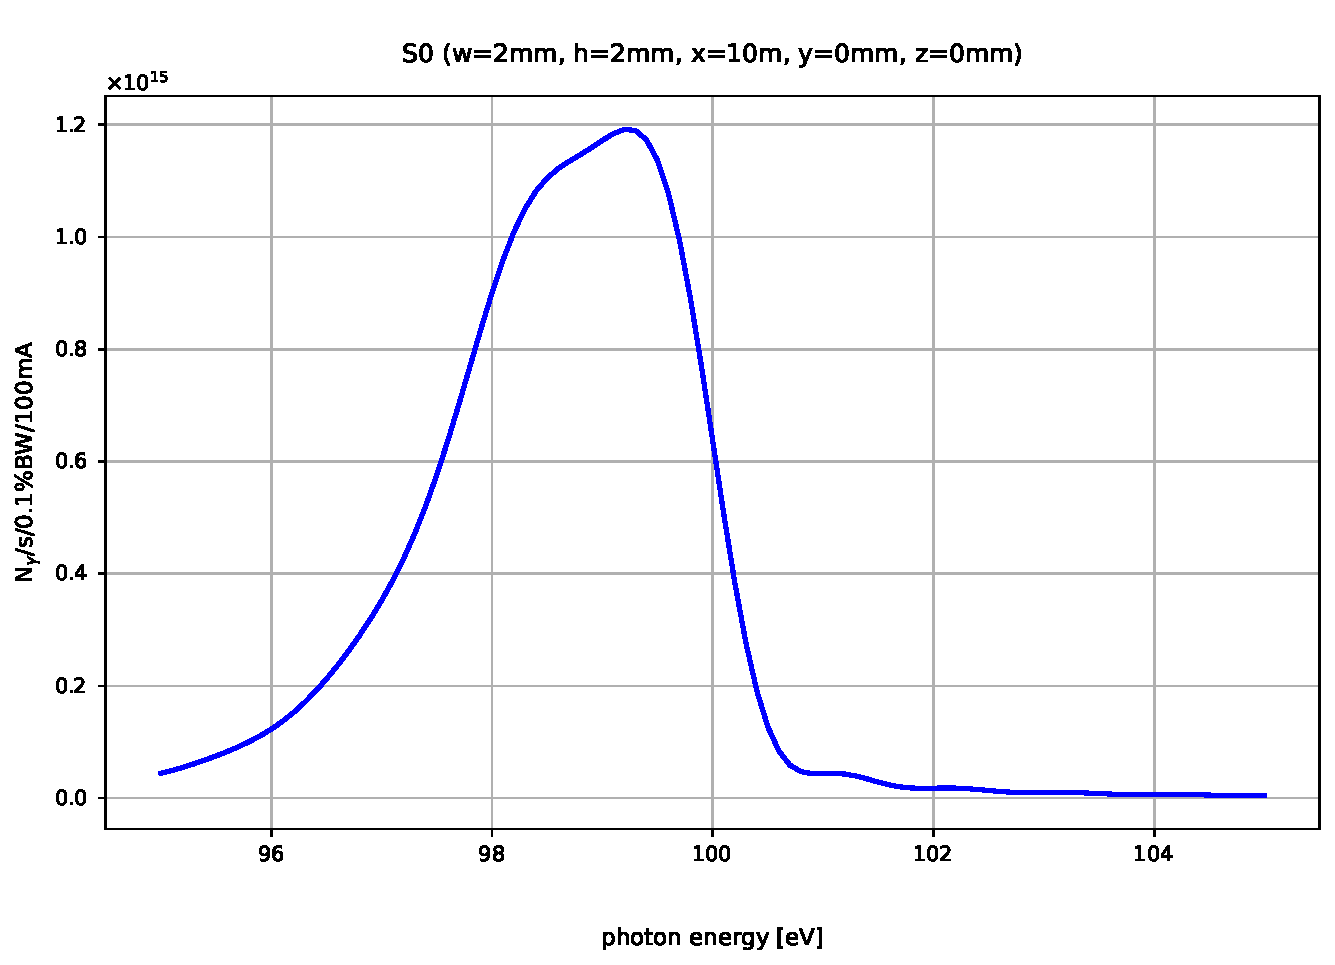
\includegraphics[width=0.7\textwidth]
   {pictures/flux.pdf}
   \caption{Flux of Undulator}
   \label{gsfig3}
\end{figure}

Press the \gti{Spectra} button, select \gite{Plot/Flux/Stokes/S0}. The
flux of the Stokes parameter \git{S0} through the rectangular pinhole
as calculated by \urp is plotted (Fig. \ref{gsfig3}).

\begin{figure}[htb]
   \centering
   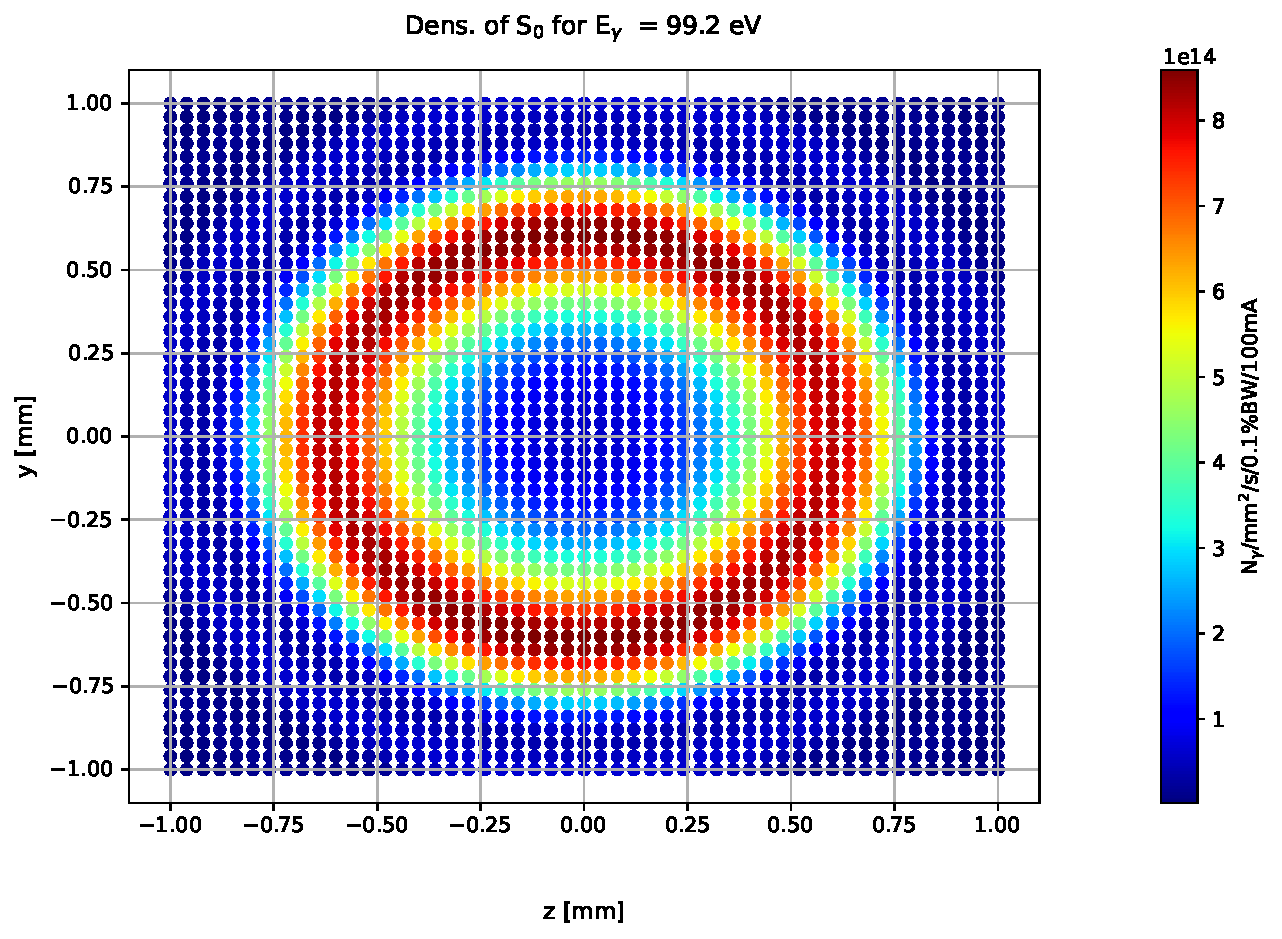
\includegraphics[width=0.7\textwidth]
   {pictures/fdpin.pdf}
   \caption{Flux-density Distribution}
   \label{gsfig4}
\end{figure}

Now, we select
\gti{Spectra/Plot/Distributions in Pinhole/Stokes/S0}
and see the flux-density distribution of \gti{S0}. The photon energy is
selected to show the distribution for the photon energy which the
maximum flux trough the pinhole.

To step through the photon energies, the arrows of the keyboard can be
used. The photon energy can also be selected from the menu

\cbox{\gti{Spectra/Plot/Distributions in Pinhole/Select E\_photon}
}



%\include{ex77} % User interfaces

\include{bibliography}
\end{document}
